\begin{frame}{Abordagem}
    
\begin{figure}
    \centering
    \begin{small}
    \begin{equation}
        \begin{split}
        \textrm{Input Layer} & \Rightarrow [ (\textrm{Convolution} \rightarrow \textrm{Batch Normalization})\cdot i\\
         &\quad \Rightarrow (\textrm{Pooling} \rightarrow \textrm{Dropout})\cdot j]\cdot k \\
         &\quad \Rightarrow [\textrm{Fully Connected} \rightarrow \textrm{ReLU}]\cdot \ell \\
         &\quad \Rightarrow \textrm{Flatten} \Rightarrow \textrm{Output Layer}
        \end{split}
    \end{equation}
    \end{small}
    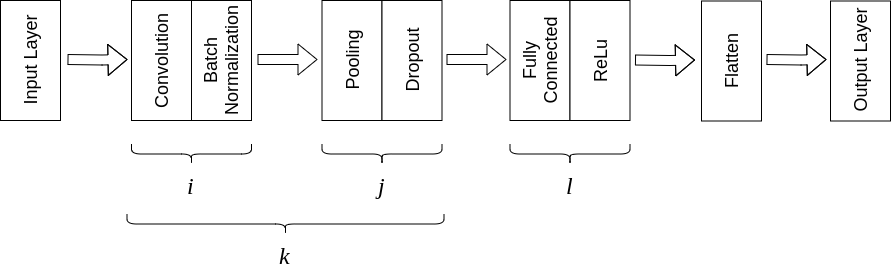
\includegraphics[width=1.0\linewidth]{img/cnn_build.png}
    \caption{Construção de modelos convolucionais.}
\end{figure}
    
\end{frame}